% Chapter 4

\chapter{Project Implementation and Simulation} % Write in your own chapter title
\label{Chapter3}
\lhead{} % Write in your own chapter title to set the page header

\section{Simulation Setup}
\subsection{Application in Communication Systems}
\subsubsection{OFDM Systems}
Firstly, the data is generated in Matlab for traditional OFDM frames. There are 64 subcarriers. The data and pilot bits, both of size 128, are generated independently and are then mapped onto QPSK modulation scheme resulting in sequences of size 64 symbol. After converting them to time-domain by taking their 64-point IFFT,  the cyclic prefix of size 16 symbols is added to both sequences after which they are concatenated. The frame of size 180 symbols is convolved with the channel impulse response, and then the Additive White Gaussian Noise is added to it. The cyclic prefix is then removed, and the pilot and data sequences are extracted. The resulting frame size of 128 symbols is ready for analysis.\\
We investigate three techniques used to recover the original data:
\begin{enumerate}
\item \textbf{Least Squares (LS) Estimation:} In this approach, the pilots are explicitly used for Channel State Information (CSI) estimation. The DFT of the channel is obtained by dividing the 64-point FFT of the pilot in the received frame by the 64 point FFT of the transmitted frame. The estimated modulated data is then obtained by dividing the 64-point FFT of the data portion from the received frame and the estimated DFT of the channel impulse response. The estimated modulated data can then be mapped back to 128 bits using QPSK constellation diagram.
\item \textbf{Time Domain Processing:} This is similar to the above-mentioned scheme except for the method of estimating H. Using our assumption on the number of channel taps, the convolution can be used to derive a matrix equation linking the channel impulse response, transmitted pilot sequence, and the received pilot sequence. Once h[n], its DFT can be computed, and the remainder of the process is the same as before.
\item \textbf{Deep Learning:} Here, we use a neural network whose architecture is explained in the diagrams below. The neural network is trained using Keras libraries for Tensorflow in python.  The details of the Neural Network Architecture are illustrated in Figure \ref{fig:comm_16_bit} and Figure \ref{fig:comm_128_bit}.
\end{enumerate}
\begin{figure}[htbp]
  \centering
  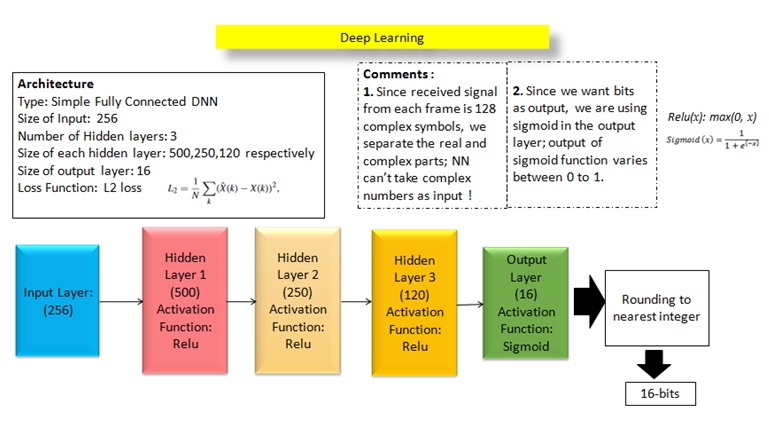
\includegraphics[width=\textwidth]{./Figures/comm_16_bit.png}
  \caption{A single Neural Network block to recover 16 bits}
  \label{fig:comm_16_bit}
\end{figure}
\begin{figure}[htbp]
  \centering
  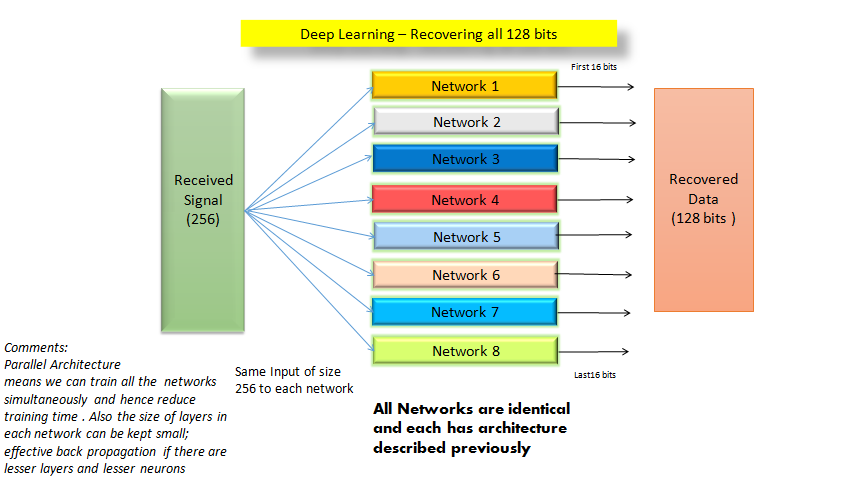
\includegraphics[width=\textwidth]{./Figures/comm_128_bit.png}
  \caption{The whole architecture that recovers all 128 bits}
  \label{fig:comm_128_bit}
\end{figure}
\subsubsection{NOMA Systems}
Using the structure for simulation for OFDM system as a skeleton, we extend our work to Non-Orthogonal Multiple Access (NOMA) system. We keep our work restricted to 2 users only. However, since the interference from two users increases the complexity of the problem at hand, we start with 16 subcarriers and a 3 tap channel to observe the trends, and then simulate for 64 subcarriers and 8 tap channel systems to confirm those trends.\\
The frame structure for NOMA is sufficiently similar to the one for OFDM system. For 16 subcarrier system, 32-bit data is converted to 16 complex symbols using QPSK modulation. Then 16 point IFFT is carried out on these symbols. Moreover, as in the case of OFDM, the pilot bits, equal in length to the data bits (true for most of our work) is QPSK modulated and converted to time-domain. The pilot is then concatenated with time domain data. However, this time space is reserved for the pilot of the other user. This ensures that while the data of the two users are non-orthogonal, the pilots are orthogonal in time. This is illustrated in figure \ref{fig:comm_noma}.\\
\begin{figure}[htbp]
  \centering
  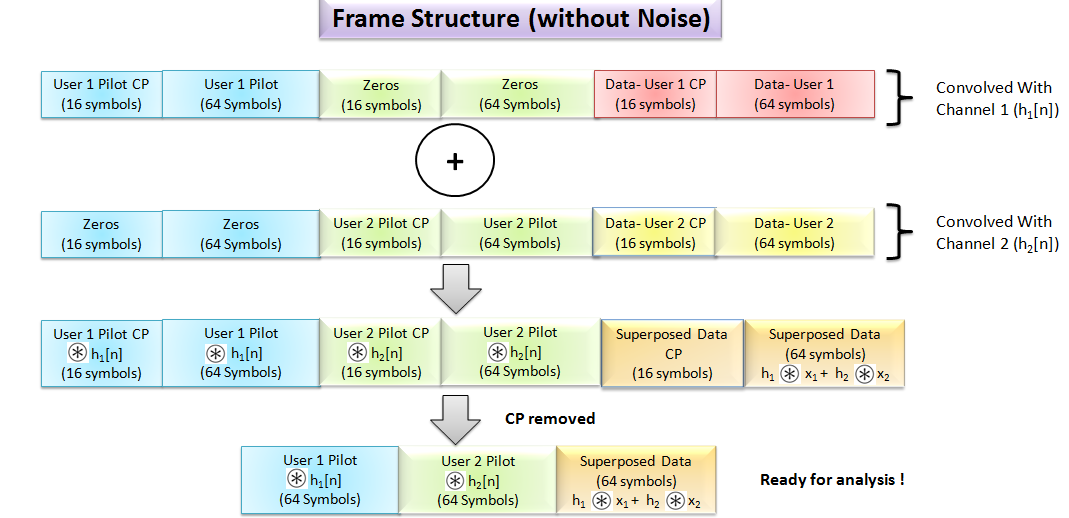
\includegraphics[width=\textwidth]{./Figures/comm_noma.png}
  \caption{Frame Structure for NOMA system: the pilot symbols are preserved despite interference}
  \label{fig:comm_noma}
\end{figure}
After interference, Gaussian noise is added to signal before it is passed onto the receiver. Unless otherwise specified, the simulations must be assumed to have been carried out at $20$ SNR. \\
The method for theoretical estimation of BER is somewhat different than the one used for OFDM systems. As before, we estimate the DFT of the channel impulse response using the pilots. We then use Maximum Likelihood estimation at a subcarrier level in frequency domain to infer which of the four possible symbols was transmitted. This can be illustrated in the following equations:\\
$$Y_{(data)}=H_1X_{1(data)}+H_2X_{2(data)}+Z$$
where,\\
$$X_1,X_2\in[e^{j(2k+1)\frac{\pi}{4}}] \mid k\in\{-2,-1,0,1\}$$
$$F^{-1}(Z)\in \mathcal{N}(0,\sigma^2)$$
The Conditional Distribution on $Y$ is given by:\\
$$f(Y\mid X_1,X_2,H_1,H_2,\sigma^2)\propto e^{-\frac{|Y-H_1X_1-H_2X_2|^2}{2\sigma^2}}$$
$$\implies \hat{X}_1 = \arg \max_{x_1\in QPSK}f(Y\mid X_1=x_1)=\arg \max_{x_1\in QPSK}\sum_{x_2\in QPSK}f(Y\mid X_1=x_1,X_2=x_2)$$
$$\implies \hat{X}_1 = \arg \max_{x_1\in QPSK}\sum_{x_2\in QPSK}e^{-\frac{|Y-H_1x_1-H_2x_2|^2}{2\sigma^2}}$$
Similarly,\\
$$\hat{X}_2 = \arg \max_{x_2\in QPSK}\sum_{x_1\in QPSK}e^{-\frac{|Y-H_1x_1-H_2x_2|^2}{2\sigma^2}}$$

To get a tighter theoretical limit on the BER, we also used separately the actual CSI (stored in a csv file) rather than the CSI estimate obtained from the pilots. \\
As far as the Deep Learning architecture is concerned, we investigated several models including the auto-encoders. However, the architecture that gave us the best results was merely a modification of the Dense Neural Network used in the single user case. We carried out our experiments for 16- Subcarrier systems and 64-Subcarrier Systems, architecture for which is shown in figure \ref{fig:comm_nomaarch}
\begin{figure}[htbp]
  \centering
  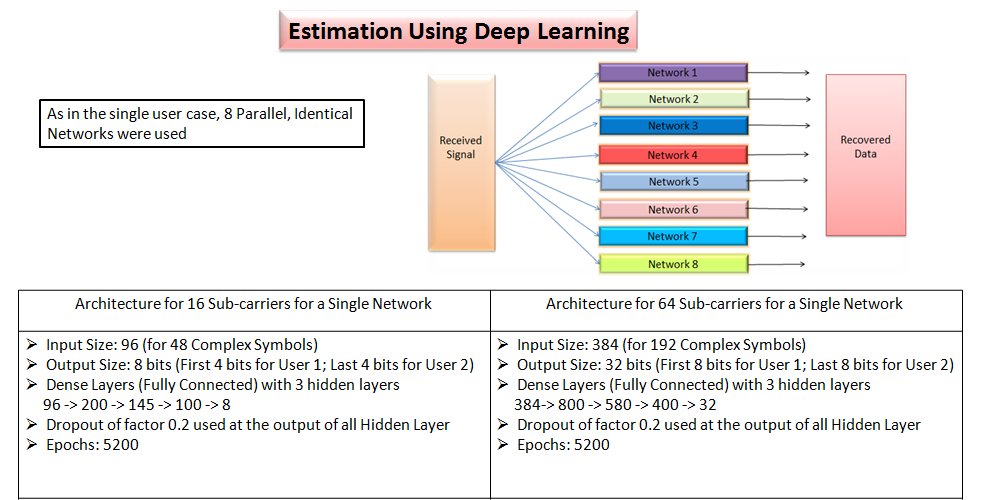
\includegraphics[width=\textwidth]{./Figures/comm_nomaarch.png}
  \caption{Deep Learning architectures used for NOMA systems}
  \label{fig:comm_nomaarch}
\end{figure}
\subsection{Application in Bioinformatics}
For this application, we first need to understand the structure of the data, and then we will move onto devising architectures for End-to-End Deep Learning. 
\subsubsection{Struture of mPower Data}
The mPower data \cite{bot2016mpower} is consists of four types of activities: Walking, Voice, Tapping and Memory. Figure \ref{fig:park_flow} illustrates the structure of mPower data. For our purposes, we limit our attention to Voice data. These four types of activities are specifically designed to trigger Parkinson's symptoms response. Each activity is recorded via the following processes:
\begin{itemize}
\item \textbf{Walking}: Subjects walk 10 steps with a phone in their pocket. Phone's Gyroscopic measurements are recorded during the whole activity. This activity is intended to capture irregularities in walking if any.
\item \textbf{Voice}: Subjects record 10 seconds of voice into the microphone of their cell-phone. This data is intended to capture the jitter or shimmer in the voice if any.
\item \textbf{Tapping}: Subjects tap on two points on the phone repeatedly. The tapping positions and intervals are recorded. This data is intended to record tremor in hand motions if any.
\item \textbf{Memory}: Subjects play a guessing game. In this game, the results of pattern matching are recorded. This activity is intended to capture if the memory is in good shape since one of the symptoms of Parkinson's is loss of memory.
\end{itemize}
\begin{figure}[htbp]
  \centering
  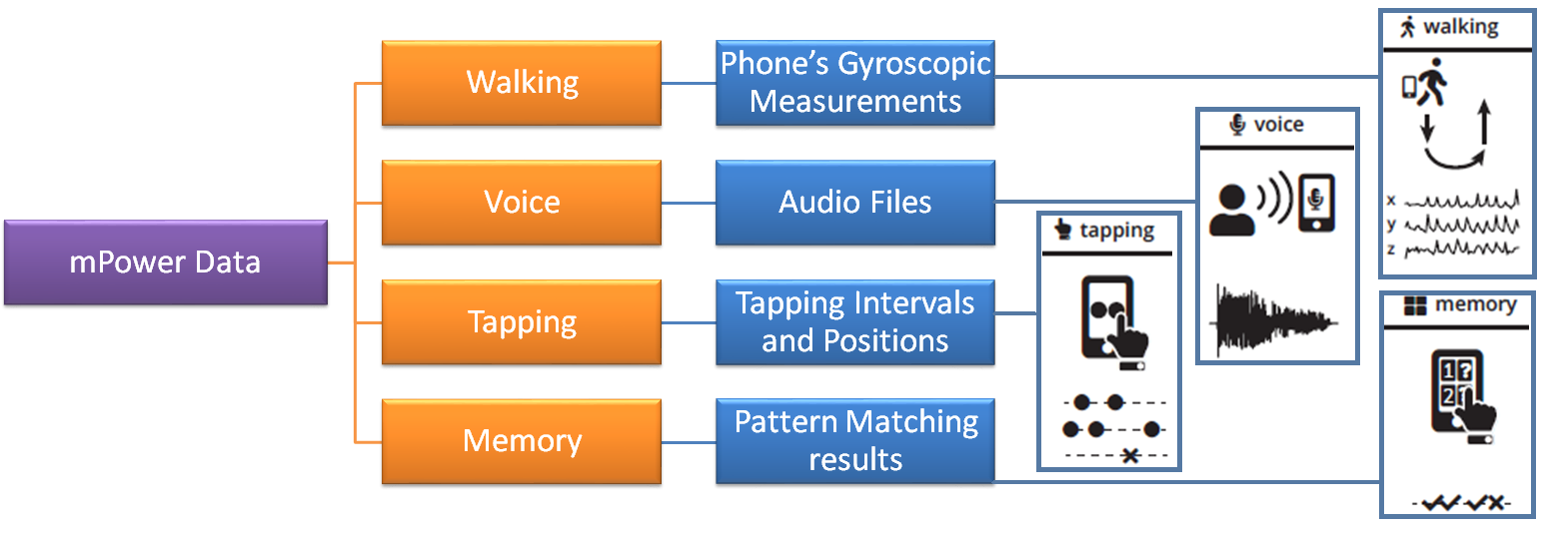
\includegraphics[width=\textwidth]{./Figures/mpower_data.png}
  \caption{The Structure of mPower Data}
  \label{fig:park_flow}
\end{figure}

\subsubsection{Structure of Voice Data}
The voice data contains 65,022 audio files in total which are organized on the basis of the time of their recording as illustrated by Figure \ref{fig:park_time}. We ignored the recordings of Parkinson's patients done just after medication, as we believe that those recordings would not provide information about Parkinson's symptoms as Parkinson's medications, suppress these symptoms \cite{schwab2018phonemd}.
\begin{figure}[htbp]
  \centering
  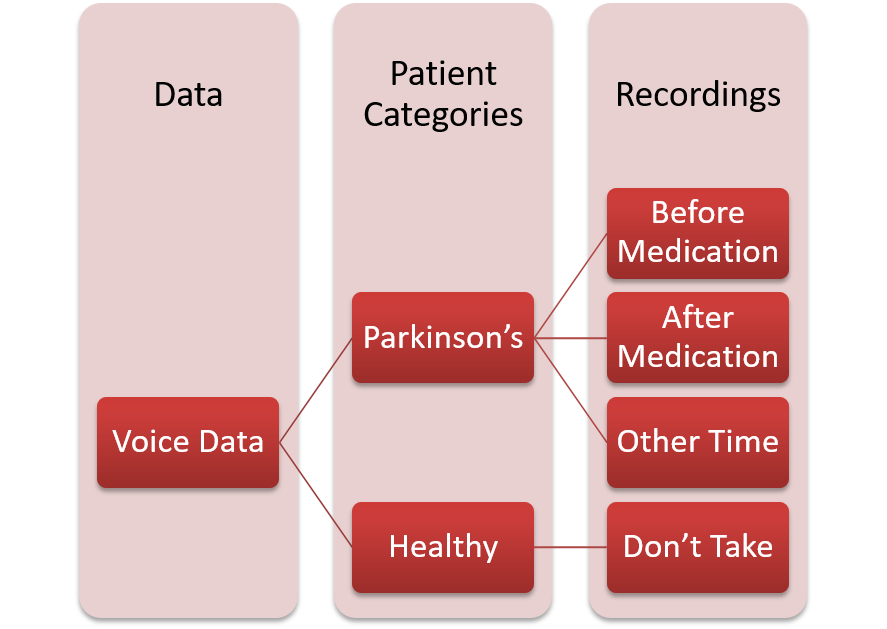
\includegraphics[width=\textwidth]{./Figures/park_time.png}
  \caption{Different types of recordings in Voice Data}
  \label{fig:park_time}
\end{figure}

However, the data available to us is imbalanced in terms of the number of people participating in the study. We observe that only 20\% of the people are clinically diagnosed by Parkinson's Disease, while an overwhelming 58\% of the recordings are attributed to that 20\ % of the people. This means that on average, people with Parkinson's have recorded more audio files as compared to Healthy people as illustrated in Figure \ref{fig:park_dist}.\\
\begin{figure}[htbp]
  \centering
  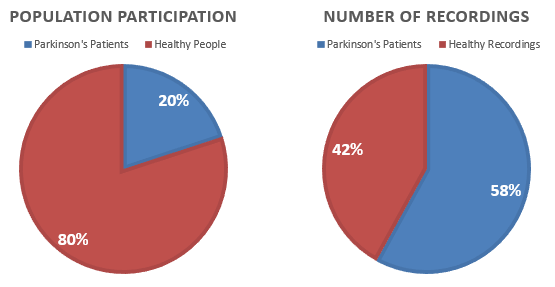
\includegraphics[width=\textwidth]{./Figures/park_dist.png}
  \caption{The Vioce Data Distribution according to PD indication}
  \label{fig:park_dist}
\end{figure}
\subsubsection{Initial Investigation with Machine Learning Models}
Initially, we assumed every recording sample independent of each other and designed a recording-level classifier. The pipeline designed for such a classifier is illustrated in Figure \ref{fig:park_pipeline}.
\begin{figure}[htbp]
  \centering
  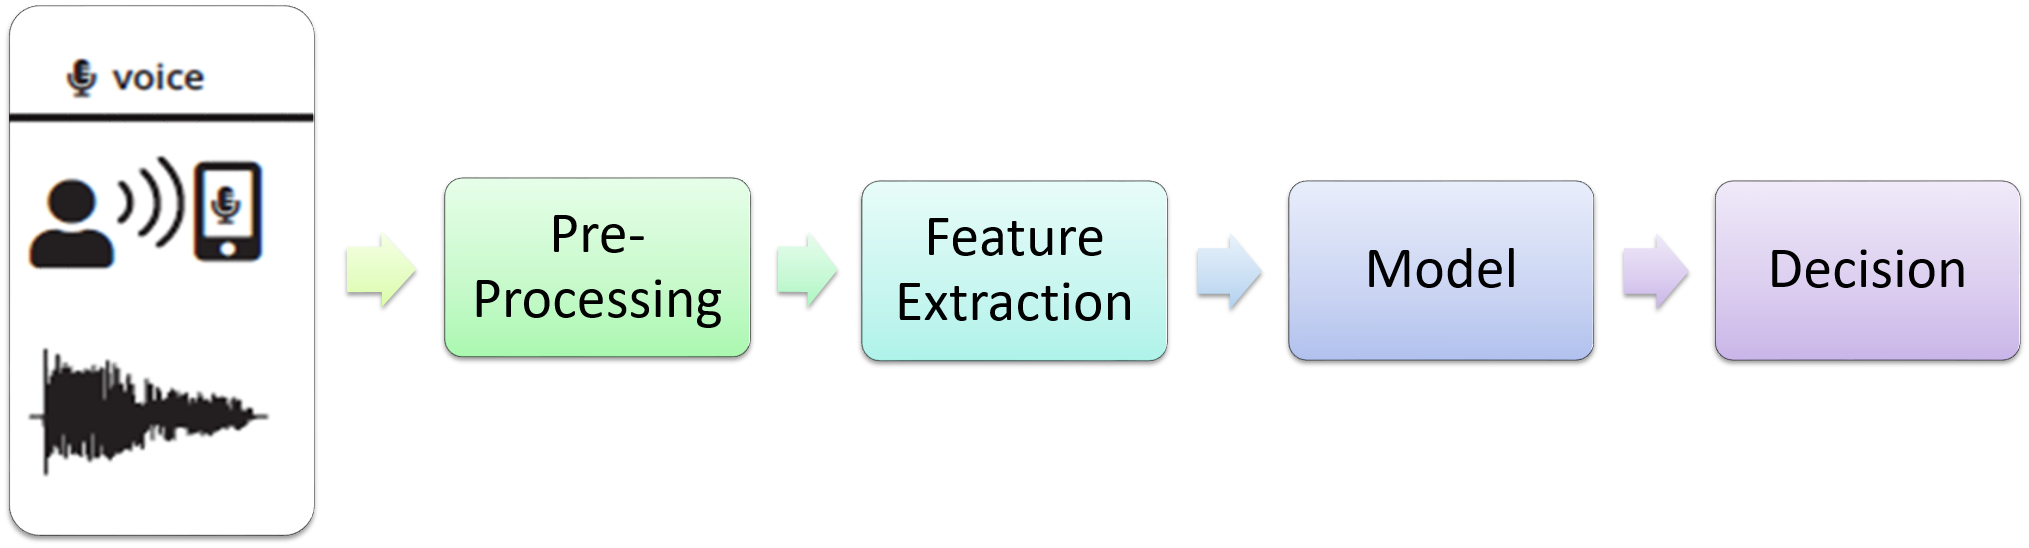
\includegraphics[width=\textwidth]{./Figures/park_pipeline.png}
  \caption{Initial Pipleline Designed for a Recording-level Classifier}
  \label{fig:park_pipeline}
\end{figure}
The following features were used for training these classifiers:
\begin{itemize}
\item Detrended fluctuation analysis \cite{arora2015detecting}
\item Mean Teager-Kaiser energy operator \cite{arora2015detecting}
\item Mel-Frequency Cepstal Co-efficients \cite{arora2015detecting}
\end{itemize}
By training these classifiers, we were able to achieve an Area Under Curve measure of 0.88 as illustrated in Figure \ref{fig:park_ini_res}, but our assumptions were wrong are there was high correlation present between two  audio-files recorded by the same patient and treating them as independent was misleading.
\begin{figure}[htbp]
  \centering
  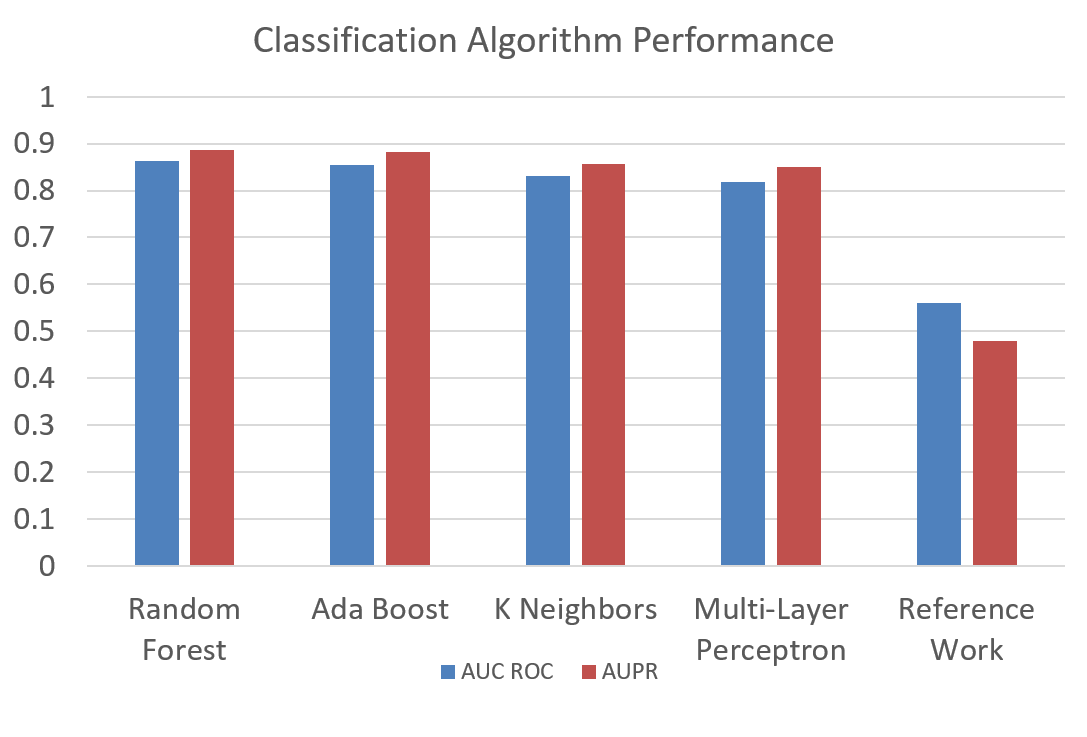
\includegraphics[width=\textwidth]{./Figures/park_ini_res.png}
  \caption{Results of Machine Learning Algorithms with Incorrect Assumption of Independence}
  \label{fig:park_ini_res}
\end{figure}
\subsubsection{Selection of a Fixed Number of Recordings per Person}
After the correction of our assumption of independence, we limited all the recordings from one particular person to either train set or the test set. Hence, a high correlation between two recordings does not affect our performance measures as all of those recordings are located entirely on one side of the split. It turns out when we limit all the recordings by one patient into either test or train dataset; the metrics drop rapidly.

The contribution of recordings by different people is very asymmetric. Some people have too many recordings, some too few. This causes a bias when training a recording level classifier as well as a person level classifier. As shown in Figure \ref{fig:park_asymm}, we see that the mode number of recordings is 3. Almost 31\% of the people have done 3 recordings, and the mean number of recordings is 11.57. 
\begin{figure}[htbp]
  \centering
  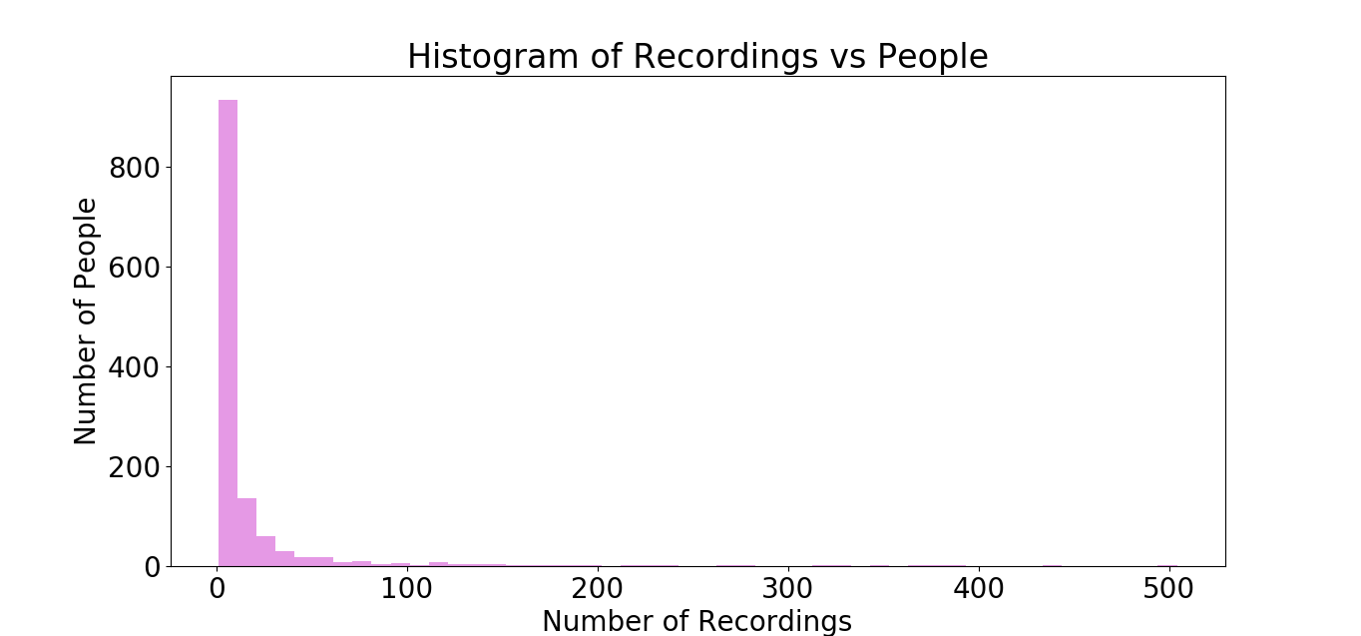
\includegraphics[width=\textwidth]{./Figures/park_asymm.png}
  \caption{Asymmetry in the Number of Recordings done by Different People}
  \label{fig:park_asymm}
\end{figure}
Therefore, we devise a policy of selecting a fixed number (let's say $k$) of recordings per person. This is done for the following reasons:
\begin{itemize}
\item People with lesser number of recordings become under-represented and provide us very less information.
\item A large number of recordings from the same person provides redundant information as the correction between two recordings by the same person is very high. This costs us in the form of un-required computation.
\end{itemize}
Therefore, we implemented this selection and tested our performance measure by selecting 2,3,4 and 5 number of recordings per person for each architecture. 
\subsubsection{Spline Convolutional Neural Network Architecture}
We use a deep neural network architecture \cite{balestriero2018spline} to classify the recordings because this architecture was designed to detect and learn features for audible data. The detailed structure for such an architecture is given in Figure \ref{fig:spline_cnn}.
\begin{figure}[htbp]
  \centering
  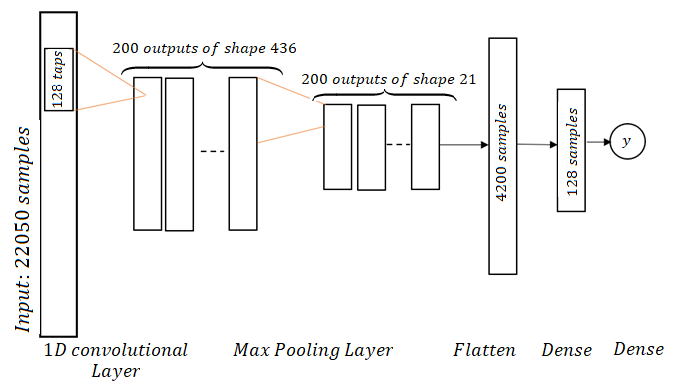
\includegraphics[width=\textwidth]{./Figures/spline_cnn.png}
  \caption{The Architecture of Spline Convolutional Neural Network}
  \label{fig:spline_cnn}
\end{figure}

The spline CNNs are a special form of regular CNNs with the change that convolutional filters are initialized as band-limited filters with several center frequencies covering the whole Frequency-space. The CNN is called spline CNN because Hermite-cubic splines are used for filter construction. The filters are constructed by first designing 1 `mother-filter' in Frequency Domain and then shifting it to cover the whole Frequency range. In our case, we use a filter of 100 Hz Bandwidth and shift it with a frequency of $\sim$10 Hz to make 200 band-limited filters. The sampling frequency we use is 2205 Hz. These 200 filters are initialized as convolutional filters in our network and then learned as we train the network. For illustration, two sample filters out of the 200 filters have been shown in Figure \ref{fig:twofils}
\begin{figure}
\centering
\parbox{6cm}{
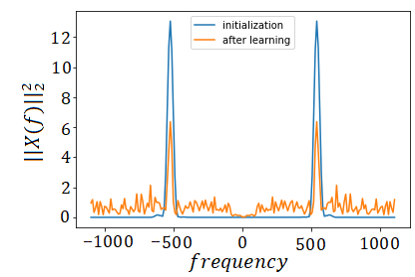
\includegraphics[width=6cm]{./Figures/park_fil1.png}
%\caption{First.}
\label{fig:2figsA}}
\qquad
\begin{minipage}{6cm}
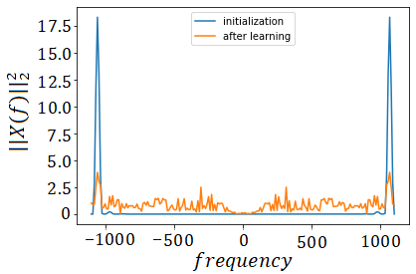
\includegraphics[width=6cm]{./Figures/park_fil2.png}
%\caption{Second.}
\label{fig:2figsB}
\end{minipage}
\caption{Sample filters for Spline-CNN}
\label{fig:twofils}
\end{figure}

\subsubsection{Evidence Aggregation Model (EAM)}
We introduced another Deep Learning Model into our pipeline to output a final prediction for each person based upon their predictions from the recording-based classifier. This updates our pipeline to the one shown in Figure \ref{fig:new_pipe}
\begin{figure}[htbp]
  \centering
  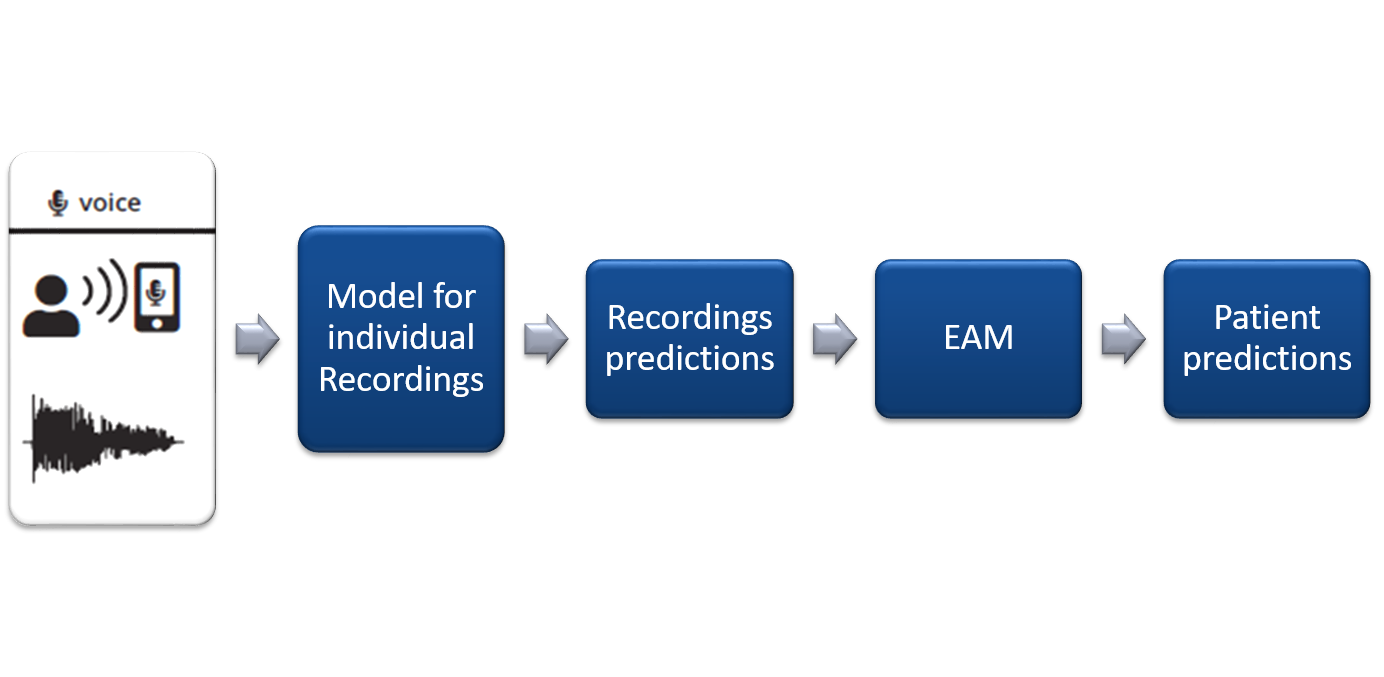
\includegraphics[width=\textwidth]{./Figures/new_pipe.png}
  \caption{New PipeLine Model after adding Evidence Aggregation Model}
  \label{fig:new_pipe}
\end{figure}
EAM is implemented as a Deep Bi-directional LSTM network, as shown in Figure \ref{fig:eam}. The work of EAM was to aggregate results from more than one models as we move towards other activities as well. However, for this setting, where we are only working with the voice data, the EAM converges to mode function.
\begin{figure}[htbp]
  \centering
  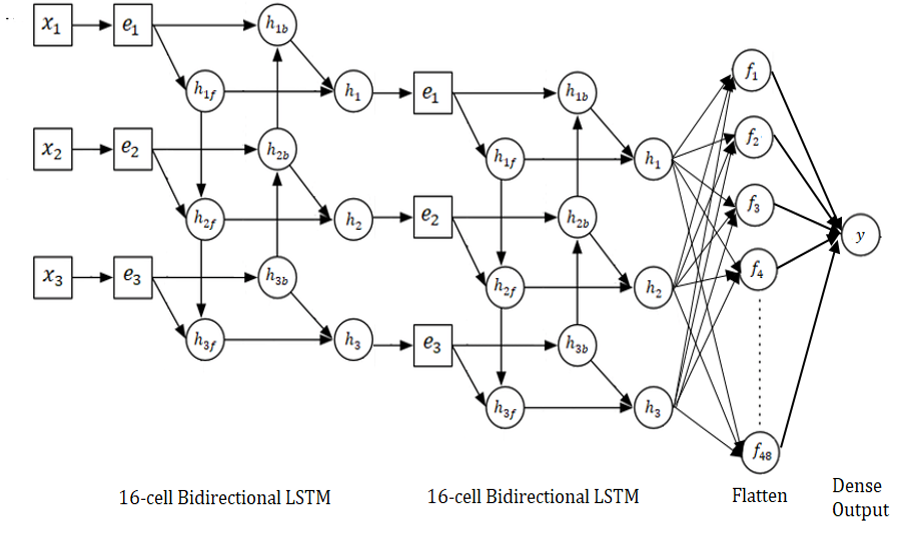
\includegraphics[width=\textwidth]{./Figures/eam.png}
  \caption{Structure of Evidence Aggregation Model}
  \label{fig:eam}
\end{figure}
\section{Simulation Results}
\subsection{Application in Communication Systems}
\subsubsection{OFDM Systems}
\begin{figure}[htbp]
  \centering
  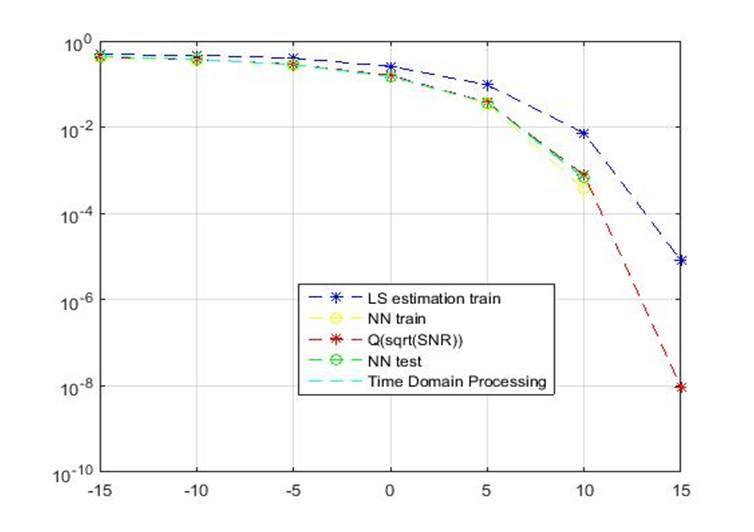
\includegraphics[width=\textwidth]{./Figures/awgn_results.png}
  \caption{Results for AWGN Channel}
  \label{fig:awgn_results}
\end{figure}
Figure \ref{fig:awgn_results} shows results for a single tap channel with Additive White Gaussian Noise (AWGN). The training data consisted of 50,000 messages while testing data consisted of 10,000 messages. The channel was unchanging across frames.  \\
We can see that Least Squares (LS) estimation fares the worst while time domain processing fares better since it utilizes the knowledge of number of channel taps used. We see that Neural Network performed the best and performed at par with Theoretical limit given by:\\
$$Q(\sqrt{10^{\frac{SNR(dB)}{10}}})$$
\begin{figure}[htbp]
  \centering
  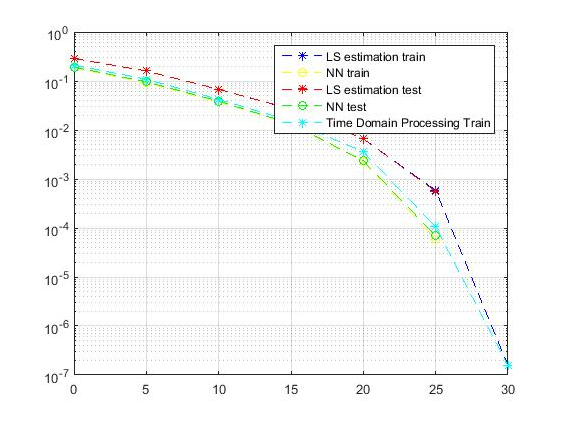
\includegraphics[width=\textwidth]{./Figures/real_8tap_res.png}
  \caption{Results for 8 tap real channel which is unchanging across frames}
  \label{fig:real_8tap_res}
\end{figure}
Figure \ref{fig:real_8tap_res} shows results for 8 tap real channel drawn from a Gaussian distribution. Again, the training data consisted of 50,000 messages while testing data consisted of 10,000 messages. The channel was unchanging across frames.  We again see that Neural Network performed the best. \\
\begin{figure}[htbp]
  \centering
  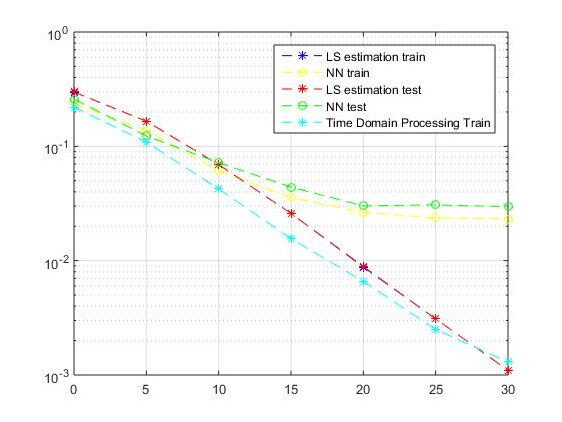
\includegraphics[width=\textwidth]{./Figures/real_8tap_chn.png}
  \caption{Results for 8-tap real channel which is changing across frames}
  \label{fig:real_8tap_chn}
\end{figure}
Figure \ref{fig:real_8tap_chn} shows results for 8-tap real channel drawn from a Gaussian distribution. As before, the training data consisted of 50,000 messages while testing data consisted of 10,000 messages. This time, the channel is changed every frame so that we have 50,000 instances of the channel. This has led to degradation in the performance of the Neural Network causing it to lag behind theoretical methods. One possible explanation could be that the neural network does not have enough examples to learn the distribution channels are drawn from.\\
\begin{figure}[htbp]
  \centering
  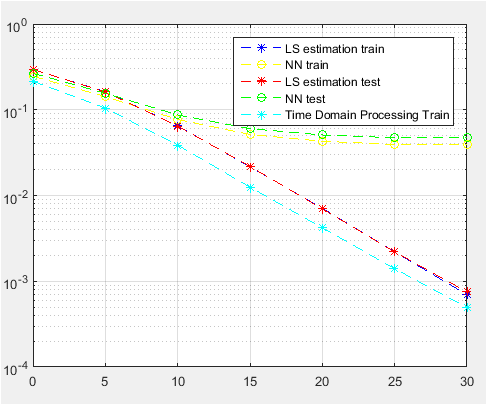
\includegraphics[width=\textwidth]{./Figures/complex_8tap_res.png}
  \caption{Results for 8 tap complex channel which is changing across frames}
  \label{fig:complex_8tap_res}
\end{figure}
Figure \ref{fig:complex_8tap_res} shows results for 8 tap complex, exponentially fading channel. Both real and imaginary parts are drawn from a Gaussian distribution and have equal energies. The training data consisted of 50,000 messages while testing data consisted of 10,000 messages. Also, the channel is changed every frame so that we have 50,000 instances of the channel. The performance of Neural Network deteriorates while the performance LS estimation and Time domain processing improves slightly.\\
\subsubsection{NOMA systems}
Since we now have to do a joint estimation of both users’ data the complexity of the problem has increased. Consequently, we had to use more neurons per layer, and we had to increase the number of epochs by a factor of 52. Therefore, we considered it prudent to carry out most of our experiments for 16 subcarrier systems and then verify them for 64 subcarrier systems.\\
\begin{table}[htbp]
  \centering
  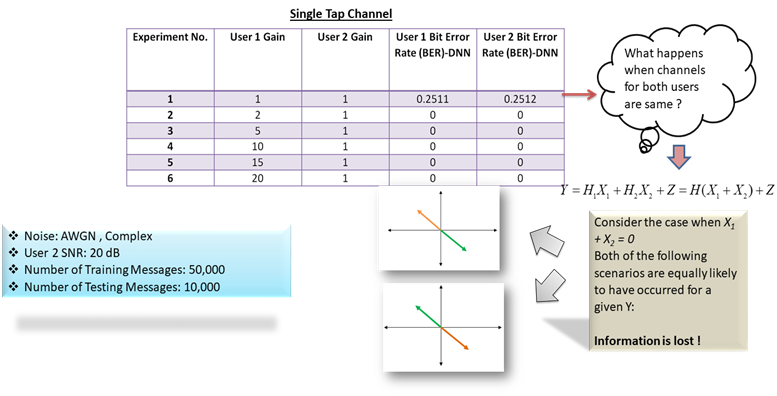
\includegraphics[width=\textwidth]{./Figures/noma_single_res.png}
  \caption{Results for Single tap Channel (NOMA)}
  \label{tbl:noma_single_res}
\end{table}
Table \ref{tbl:noma_single_res} shows results for a Single tap channel. The noise added was complex. The Signal to Noise ratio (SNR) for user 2 was maintained at 20 dB. The gain for user 1 was varied which was akin to changing its SNR. The number of training messages used was 50,000 while the number of testing messages used was 10,000. As we can see here, the neural network achieved perfect decoding of the received data. However, it was observed that when the channel for both users was same, the Neural Network failed because QPSK modulation uses sets of symbols that are $180^o$ apart in phase, that cancel out resulting in a loss of information.\\
\begin{table}[htbp]
  \centering
  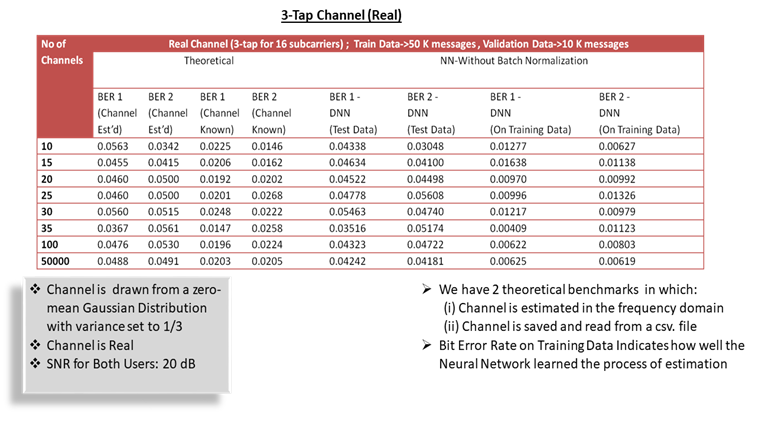
\includegraphics[width=\textwidth]{./Figures/noma_3tap_res.png}
  \caption{Results for 3-tap Real Channel (NOMA)}
  \label{tbl:noma_3tap_res}
\end{table}
\begin{figure}[htbp]
  \centering
  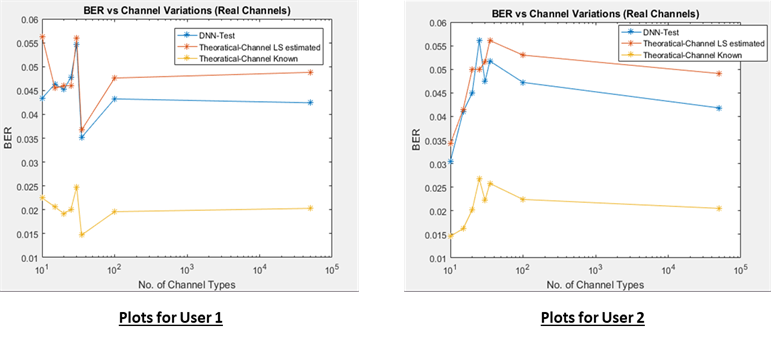
\includegraphics[width=\textwidth]{./Figures/noma_comp.png}
  \caption{Plots of BER for both users for 3-tap Real Channel against No. of Channel (NOMA)}
  \label{fig:noma_comp}
\end{figure}
Table \ref{tbl:noma_3tap_res} and Figure \ref{fig:noma_comp} demonstrate results when the number of Channel taps is increased to 3. The Channel is kept real and drawn from a zero-mean Gaussian distribution. This time, the SNR for both of the users is maintained at 20 dB. We used 2 theoretical benchmarks to gauge the performance of the Neural Network. The first method uses Least Squares Estimation in the frequency domain to estimate the channel. In the second method, the channel is saved and loaded from a .csv file and used to recover the data. Since the major hurdle in the data recovery is channel estimation, this method gives us the theoretical limit below which the bit error rate cannot possibly go. We investigated the BER against the increase in Number of Channel types or instances. The plots show that the neural network performs slightly better than the theoretical method that uses Least squares estimation of the channel. Also, we see that contrary to the case of single user detection; the neural network has also managed to learn the channel distribution as the performance of the neural network does not degrade as we increase the number of channel types. Similarly, figure \ref{fig:noma_3tap_snr} below shows that BER decreases with increasing SNR.\\
\begin{figure}[htbp]
  \centering
  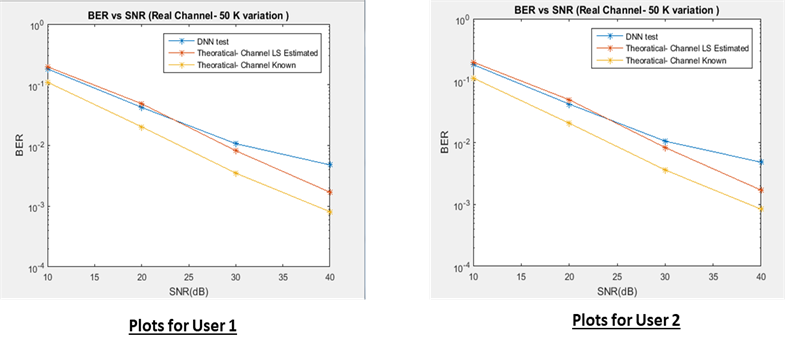
\includegraphics[width=\textwidth]{./Figures/noma_3tap_snr.png}
  \caption{Plots of BER for both users for 3-tap Real Channel against SNR (NOMA)}
  \label{fig:noma_3tap_snr}
\end{figure}
\begin{table}[htbp]
  \centering
  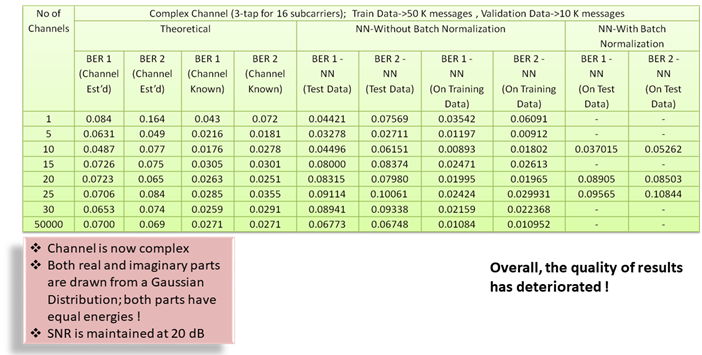
\includegraphics[width=\textwidth]{./Figures/noma_3tap_complex.png}
  \caption{Results for 3-tap Complex Channel (NOMA)}
  \label{tbl:noma_3tap_complex}
\end{table}
\begin{figure}[htbp]
  \centering
  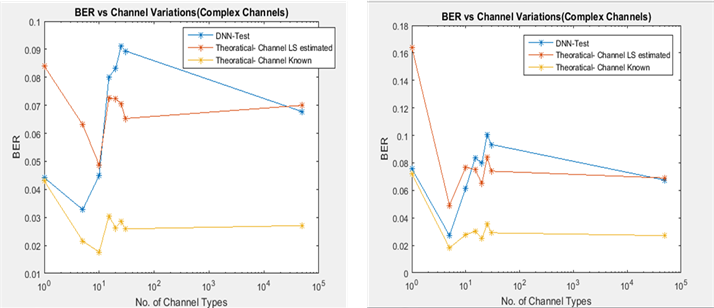
\includegraphics[width=\textwidth]{./Figures/noma_3tap_complexnochannel.png}
  \caption{Plots of BER for both users for 3-tap Complex Channel against No. of Channel (NOMA)}
  \label{fig:noma_3tap_complexnochannel}
\end{figure}
Table \ref{tbl:noma_3tap_complex} and Figure \ref{fig:noma_3tap_complexnochannel} demonstrate what happens when we make the channel complex. Both the real and imaginary parts of the channel have been drawn from a Gaussian distribution, and the energies of both parts are kept equal. We can see that the bit error rates have gone up and the overall quality of results have deteriorated. However, the Neural Network still performs at par with the theoretical method that estimates the channel using the Least Squares. \\
To confirm the robustness of our results, we extend our experiments to 64 subcarrier system, the results of which are shown in Table \ref{tbl:noma_8tap_res}. Since the Number of training, messages have been increased 10 folds, and the neurons in each layer have also been increased, the training took longer than the training in the 16-subcarrier system. Results show that the Neural Network performs slightly poorer than the theoretical methods.
\begin{table}[htbp]
  \centering
  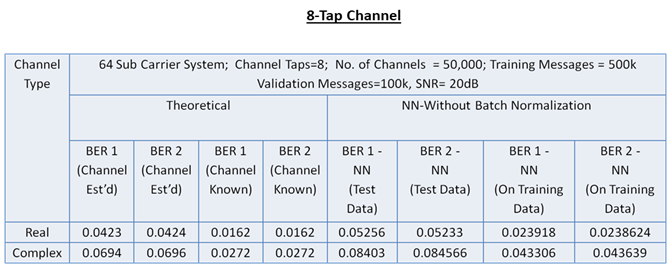
\includegraphics[width=\textwidth]{./Figures/noma_8tap_res.png}
  \caption{Results for an 8-tap complex channel varying across frames for 64 sub-carrier system}
  \label{tbl:noma_8tap_res}
\end{table}
\subsection{Application in Bioinformatics}
We compare our results to the state-of-the-art work on the same dataset by P.Schwab \cite{schwab2018phonemd} who have used Traditional Machine Learning techniques to classify between Parkinson's patients and Healthy persons.
\subsubsection{Results using Random Forest}
After the correction of our independence assumption, we were able to improve upon the reported result by using more robust hand-crafted features as shown in Figure \ref{fig:first_res}.
\begin{figure}[htbp]
  \centering
  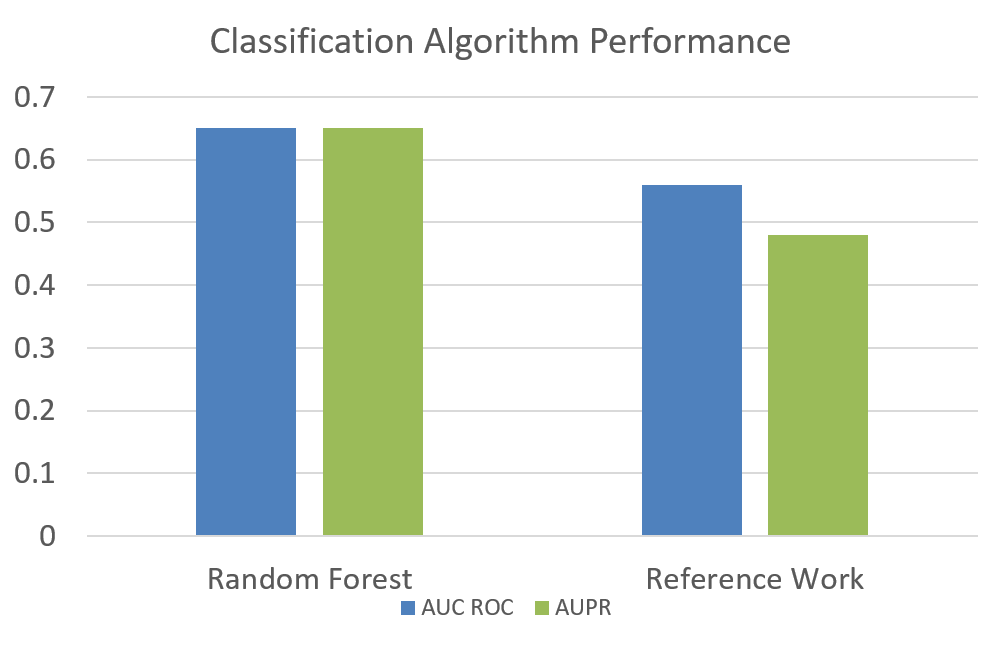
\includegraphics[width=\textwidth]{./Figures/first_res.png}
  \caption{Results from a simple Random Forest Classifier}
  \label{fig:first_res}
\end{figure}
Using Random Forest with EAM, improved our results to an AUC of 0.76 in comparison of 0.56 obtained by P.Schwab \cite{schwab2018phonemd} on Voice Data as shown in Figure \ref{fig:second_res}
\begin{figure}[htbp]
  \centering
  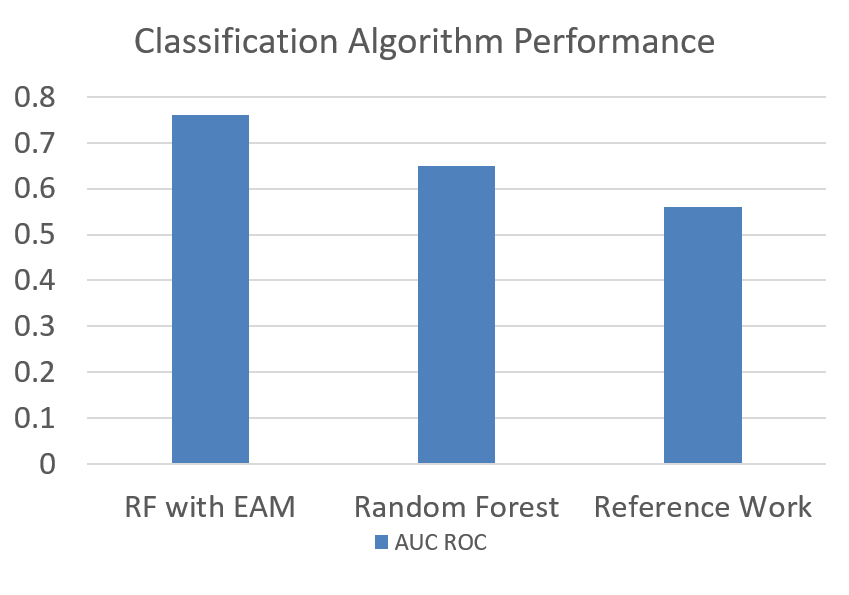
\includegraphics[width=\textwidth]{./Figures/second_res.png}
  \caption{Results from a simple Random Forest Classifier Alongwith EAM}
  \label{fig:second_res}
\end{figure}
\subsubsection{Results using Spline CNN}
The next logical step was to replace recording-level with a CNN to skip the pre-processing and feature Extraction step. This improved our measure to an AUC ROC of 0.89 with EAM for 3 recordings per patient as shown in Figure \ref{fig:third_res}
\begin{figure}[htbp]
  \centering
  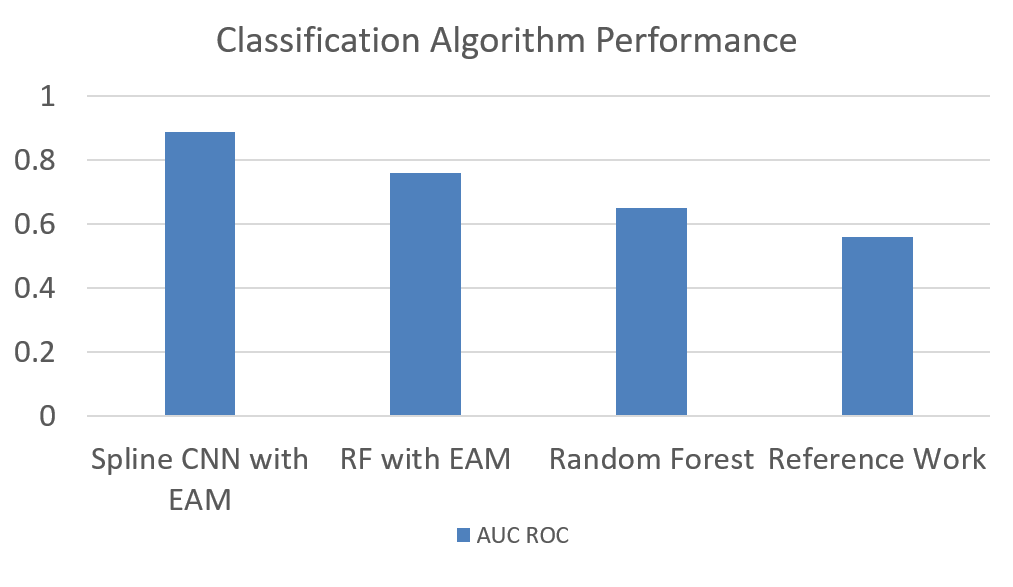
\includegraphics[width=\textwidth]{./Figures/third_res.png}
  \caption{Results from a Spline CNN Alongwith EAM}
  \label{fig:third_res}
\end{figure}
\subsubsection{Results Using Different Values of Recordings per Person}
The number of recordings per person were also changed and the results were recorded. As we can see that this change does not affect the performance very significantly,yet maximum performance was obtained at 3 recordings per person as shown in Figure \ref{fig:fourth_rse}.
\begin{figure}[htbp]
  \centering
  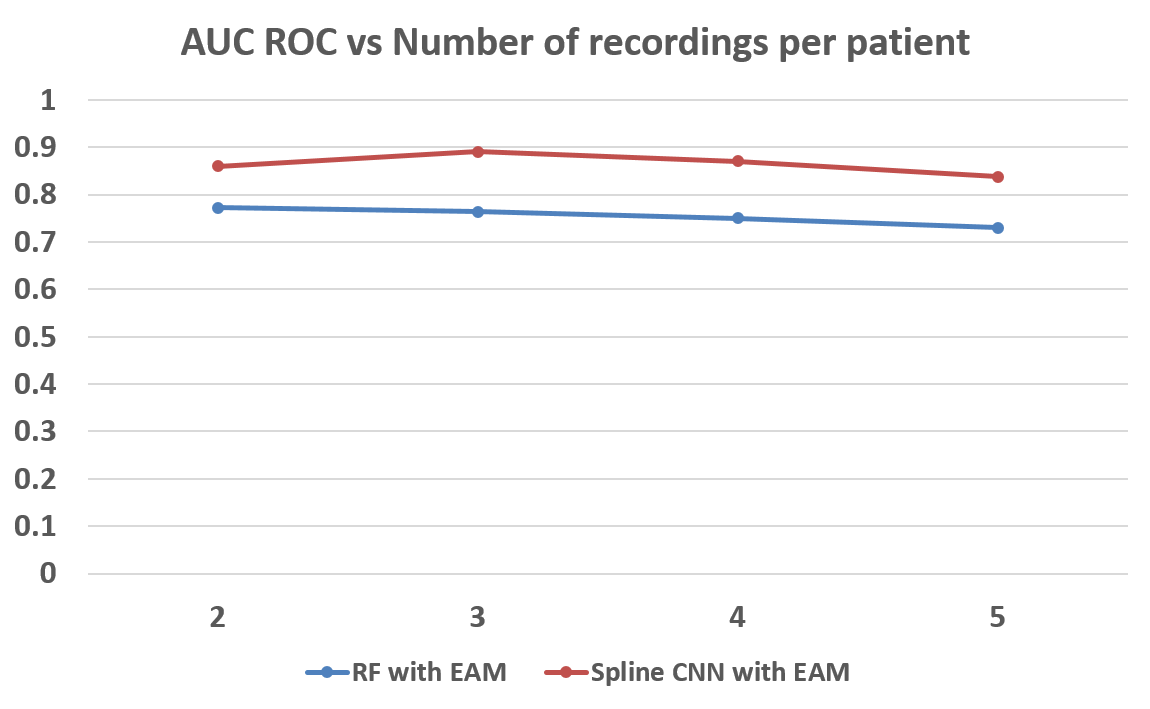
\includegraphics[width=\textwidth]{./Figures/fourth_rse.png}
  \caption{Change in Performace with Respect to Number of Recordings per Person}
  \label{fig:fourth_rse}
\end{figure}
The data composition was also changed when we changed the number of recordings per person which is illustrated in Figure \ref{fig:fifth_res}
\begin{figure}[htbp]
  \centering
  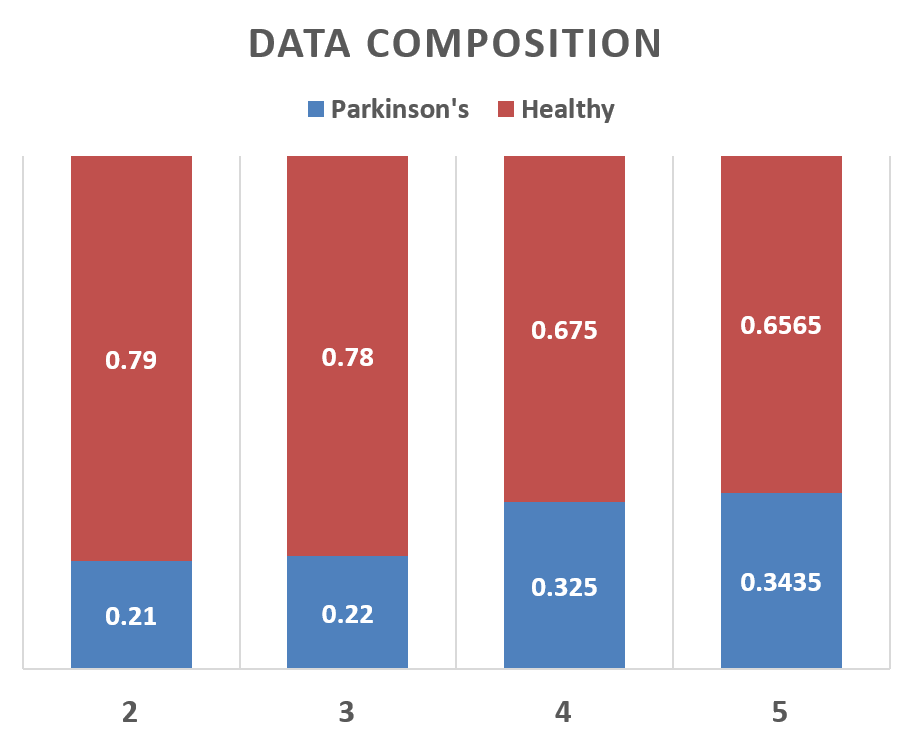
\includegraphics[width=\textwidth]{./Figures/fifth_res.png}
  \caption{Data Composition as we change the number of recordings per patient}
  \label{fig:fifth_res}
\end{figure}
\section{Result Analysis And Outlook}
\subsection{Application in Communication Systems}
The major stumbling block identified by our results is the need for training data. Our generalization error is made up of 2 components: Bias Error and Variance Error. While bias error can be decreased by making the model more complex, variance error cannot be decreased without increasing the amount of training data. For single user detection, when the channel was unvarying across frames, our neural network did not need to learn the channel distribution, and therefore a small number of training messages sufficed. However, as we increased the number of channel instances, the DNN needed to learn the underlying distribution of the channel and consequently required a large amount of training data. That is why for an unchanging, channel, our DNN performed the best, while for a changing channel it performed the worst. Table \ref{tbl:train_single_user} shows that as we increase the amount of training data, the performance of the neural network starts to improve.\\
\begin{table}[htbp]
  \centering
  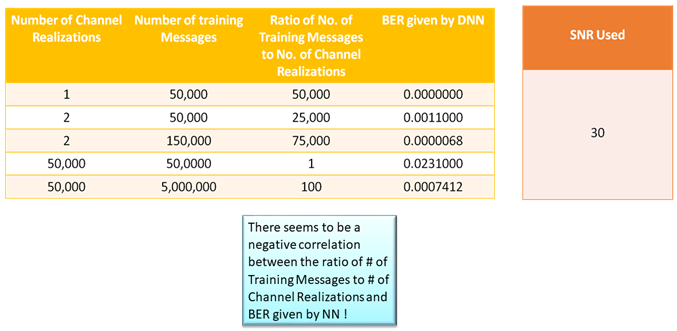
\includegraphics[width=\textwidth]{./Figures/train_single_user.png}
  \caption{Effect of increasing the Training Data for Single User Detection}
  \label{tbl:train_single_user}
\end{table}
Similarly, Table \ref{tbl:train_multi_user} convincingly suggests at lower amounts training data, the performance of the neural network is at par with the theoretical method that estimates the channel with Least Squares. However if we increase the number of training messages, the performance of the DNN improves, and it tries to approach the theoretical limit calculated by using the exact channel response which had been saved and loaded from a .csv file.  
\begin{table}[htbp]
  \centering
  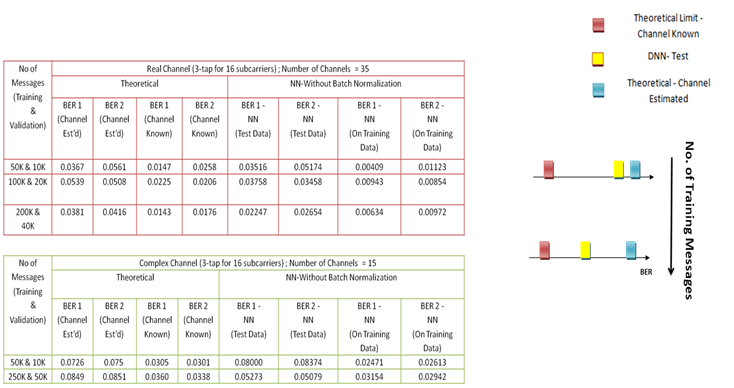
\includegraphics[width=\textwidth]{./Figures/train_multi_user.png}
  \caption{Effect of increasing the Training Data for Multi-User Detection}
  \label{tbl:train_multi_user}
\end{table}
\subsection{Application in Bioinformatics}
The major takeaway from our results is the importance of End-to-End Deep Learning as we have been able to improve quite a lot on the previous results by using the Spline-CNN. The main advantage of Spline-CNN is that it does not  need us to compute convolutional filters, but instead learns those filters based on data itself; we just initialize the filters as band-limited filters with the help of splines, and the rest is learned by the Network itself.\\
However, for End-to-End Deep Learning, here, we also face the same problem of the requirement of large amounts of data. This trend can be observed in Figure \ref{fig:fourth_rse} because as we increase the number of recordings per person, the results show a trend of decreasing performance. This is due to the decreasing amount of data we have available when we increase the number of recordings per person as there are fewer people who have recorded that many number of recordings or more. We can observe this trend in the number of recordings histogram in Figure \ref{fig:park_asymm}.